\documentclass[a4paper, 12pt]{article}


\usepackage{graphicx}
\usepackage{graphics}   
%\usepackage[utf8x]{inputenc}
\usepackage{indentfirst}
\usepackage{color}
\usepackage{xcolor}
\usepackage{graphicx}	
\usepackage{graphics} 
\usepackage{amsfonts} 
\usepackage{amsmath}
\usepackage{amssymb}
\usepackage[english]{babel}	
\usepackage{setspace}
\usepackage{comment}
\usepackage{listings}
\usepackage{lipsum}
\usepackage{mathtools}
\usepackage{caption}
\usepackage{csquotes}
\usepackage{hyperref}
\usepackage{url}
\usepackage{longtable}
\usepackage{booktabs} 
\usepackage[backend=biber,style=numeric,sorting=ynt]{biblatex}

\usepackage{tikz}
\usepackage{tikzscale}
\usetikzlibrary{babel,arrows,automata}
\usepackage[siunitx,american,cuteinductors,smartlabels]{circuitikz}


\graphicspath{{images/}}        % Caminho das imagens
\pagenumbering{arabic}          % Numeração das páginas
\everymath{\displaystyle}       % \frac{}{} tamanho ideal



\addbibresource{bib.bib}

\begin{document}
    \onehalfspacing
\begin{titlepage}
	\begin{center}
	
	\begin{figure}[!ht]
	\centering
	\end{figure}

		\vspace{15pt}
        \vspace{50pt}
        \large{Levy Gabriel da Silva Galvão}\\
		\vspace{3,5cm}
		\textbf{\Large{Experimental data acquisition and processing system for ECG signals}}
	\end{center}
	

	\vspace{1cm}
	
	\begin{center}
		\vspace{\fill}
		Natal - RN \\ October, 2021
	\end{center}
\end{titlepage}
%%%%%%%%%%%%%%%%%%%%%%%%%%%%%%%%%%%%%%%%%%%%%%%%%%%%%%%%%%%

\newpage
\begin{center}
\textbf{\Large Abstract}
\end{center}

\lipsum[1]

\begin{flushleft}
\textbf{Keywords}: oi. turo. bem.
\end{flushleft}

\pagebreak


\listoffigures
\pagebreak
\listoftables
\pagebreak

\tableofcontents
\pagebreak


    \section{Introduction}

\lipsum[1]

\pagebreak
\section{Specifications}

\subsection{Cardiac signal}

The electrical potentials of the cardiac signal are acquired by various electrodes connected in the surface of the skin of the patient. Those combined generate the cardiac signal, as can be seen in the normal wave pattern of figure \ref{fig:cardiac_signal}, with voltage differences in the order of $1 \, mV$ between given points in the body \cite{khandpur2019compendium}.

\begin{figure}[h!] 
    \centering
    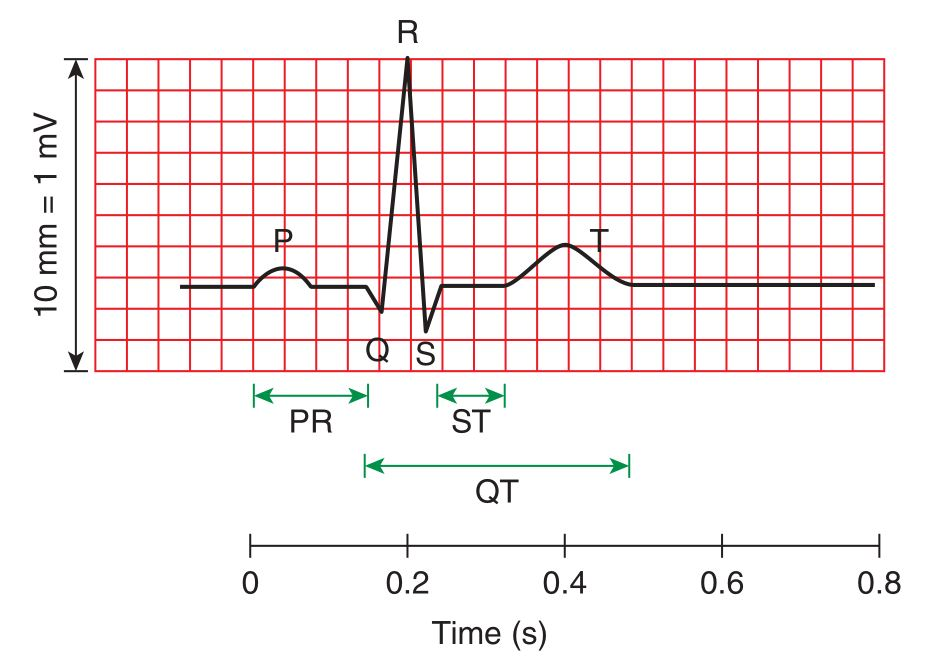
\includegraphics[width=9cm]{images/cardiac_signal.JPG}
    \caption{Normal waveform pattern of cardiac signal obtained in ECG. Source: \textcite{khandpur2019compendium}.}
    \label{fig:cardiac_signal} 
\end{figure}

Regarding the figure \ref{fig:cardiac_signal}, each letter has a proper meaning for each step in the cardiac cycle. Those are:

\begin{itemize}
    \item The P wave represents the depolarization of the atrial muscles;
    \item The QRS section is a combination of the atria repolarization between QR and the ventricles depolarization between RS;
    \item The T wave represents the repolarization of both ventricles;
\end{itemize}

The interval PR represents the actrial systole, of which the diastole lasts from R until the next P wave. The ventricular systole occurs between R until the end of the T wave and its diastole lasts until Q \cite{openstax}. 

The interval QRS representing the time taken by the heart impulse to travel from the inter ventricular system then through the walls of the ventricles is the most critical one when thinking in the design of an ECG machine since it has the higher frequency of all the cardiac signal and lasts about 0.05 to 0.1 seconds \cite{khandpur2019compendium}.

Those characteristics leads to a deeper specification of the ECG regarding the signal. \textcite{khandpur2019compendium} defines the frequency range of the signal varying from $0.05$ to $150 \, Hz$. By the Nyquist sampling theorem, it is recommended that the sampling frequency used in digitization to be at least two times the higher frequency in the signal, i.e $300 \, \text{samples}/s$. Despite this, \textcite{khandpur2019compendium} exerts that a sampling rate of $200 \, \text{samples}/s$ is satisfactory, yielding 12 to 20 samples for the QRS interval. Therefore the system designed in this work will attend to the Nyquist criteria and beyond, using a sampling frequency of $500 \, \text{samples}/s$. The disadvantage in this approach is that compared to the sampling frequency proposed by \textcite{khandpur2019compendium}, the present system will need $2.5 \times$ more space due its higher sampling frequency.

Regarding the bit resolution to store the cardiac signal, \textcite{khandpur1987handbook} suggests two approaches: to use low-noise and high-gain amplifiers, enabling the use of low-resolution 16-bit ADC; or using a low-gain amplifier with a high-resolution 24-bit ADC. The first approach will be used in this project for the sake of a more elaborated amplifier design and signal conditioning, instead just using a better ADC.

Since the arrangement of electrodes is not the main focus of this work, the system will stick with a bipolar leads arrangement. This arrangement uses two electrodes placed in the right and left arm to capture the signal and send to the input of an instrumentation amplifier and other electrode as reference placed in the left leg \cite{khandpur2019compendium}. This means that there is no need for a multiplexing system for multiples channels of electrodes, like in a typical 12-lead ECG \cite{zhang201212}.

\subsection{Associated noises}

In the chain of processing, the cardiac signal must be filtered in a way to remove certain noises and interference inherent to the data acquisition. The most common source are: interference from the power-lines (power grid) as a tone in $50/60 \, Hz$ (depending on the region of the globe); noise generated mechanically due to the contact between electrodes and skin, motion artefacts firing random derived from the patient movement and muscle contraction (voluntary or involuntary); additive white Gaussian noise (AWGN) derived from thermal sources; or electromagnetic interference from other electronics devices that can extends to the RF spectrum or higher \cite{khandpur1987handbook}.

It is essential to a ECG instrument to maintain clear of those noises and interference in a level of approximately $10 \, \mu V$ peak to peak to ensures ECG applications in diagnostics \cite{khandpur1987handbook}.

Each source of noise and interference can be treated in a specific manner.

\paragraph{Power-line interference} can be solved designing a Notch filter (reject band) with cutoff frequency set to $50/60 \, Hz$ (this project will validate the filter to $60 \, Hz$).

\paragraph{Baseline wanders and muscle contraction} are phenomena of low frequencies and they can be eliminated with the help of a high-pass filter. In the previous section the lower frequency defined to the cardiac signal was $0.05 \, Hz$, so a high-pass filter with this value as cutoff frequency should be able to remove those interference without risking rising too much the cutoff and attenuating the P or T waves \cite{khandpur2019compendium, khandpur1987handbook, murugappan2014development}. \textcite{sahin2020instrumentation} suggests the use of a $0.5 \, Hz$ cutoff frequency in a fourth order Butterworth filter, therefore allowing the use of a simpler filter with relaxed requirements and alerting that this cutoff may be tuned to meet the requirements. The $0.5 Hz$ cutoff frequency will be used in this project.

\paragraph{AWGN and electromagnetic interference} are phenomena of mainly high frequencies, therefore can be eliminated with a low-pass filter that might be designed with the anti aliasing filter. The anti aliasing filter is a analog and low order filter, but can also be used to eliminate electromagnetic interference since it has a frequency band way higher than the signal. The AWGN is uniform thought out all frequencies, so the previous high-pass filter will contribute to eliminate some of the noise. The cutoff frequency selected for this filter will be $200 \, Hz$ which comprises the signal band.

An alternative idea is to merge both low-pass and high-pass filters into a band-pass filter. The problem associated with this strategy is that it is not possible to select different filter orders to the low-pass and high-pass segment. Even though this project will stick with a band-pass filter combining the high-pass and low-pass filter cutoff frequencies, thus simplifying the circuit.

Below there is table \ref{tbl:1} showing a summary of the analog filters to be designed in further sections.

\begin{longtable}[H]{lcc}

\toprule
Filter & Cutoff frequency\\
\midrule
\endhead
Notch (analog) & $60 \, Hz$ \\
Band-pass (analog) & $0.5 \, Hz$ to $200 \, Hz$  \\
\bottomrule
\caption{Summary of filters.}
\label{tbl:1}
\end{longtable}


\pagebreak
\section{Methodology}

\subsection{System overview}

The idealized system follows the sketch of the figure \ref{fig:system}

\begin{figure}[h!] 

    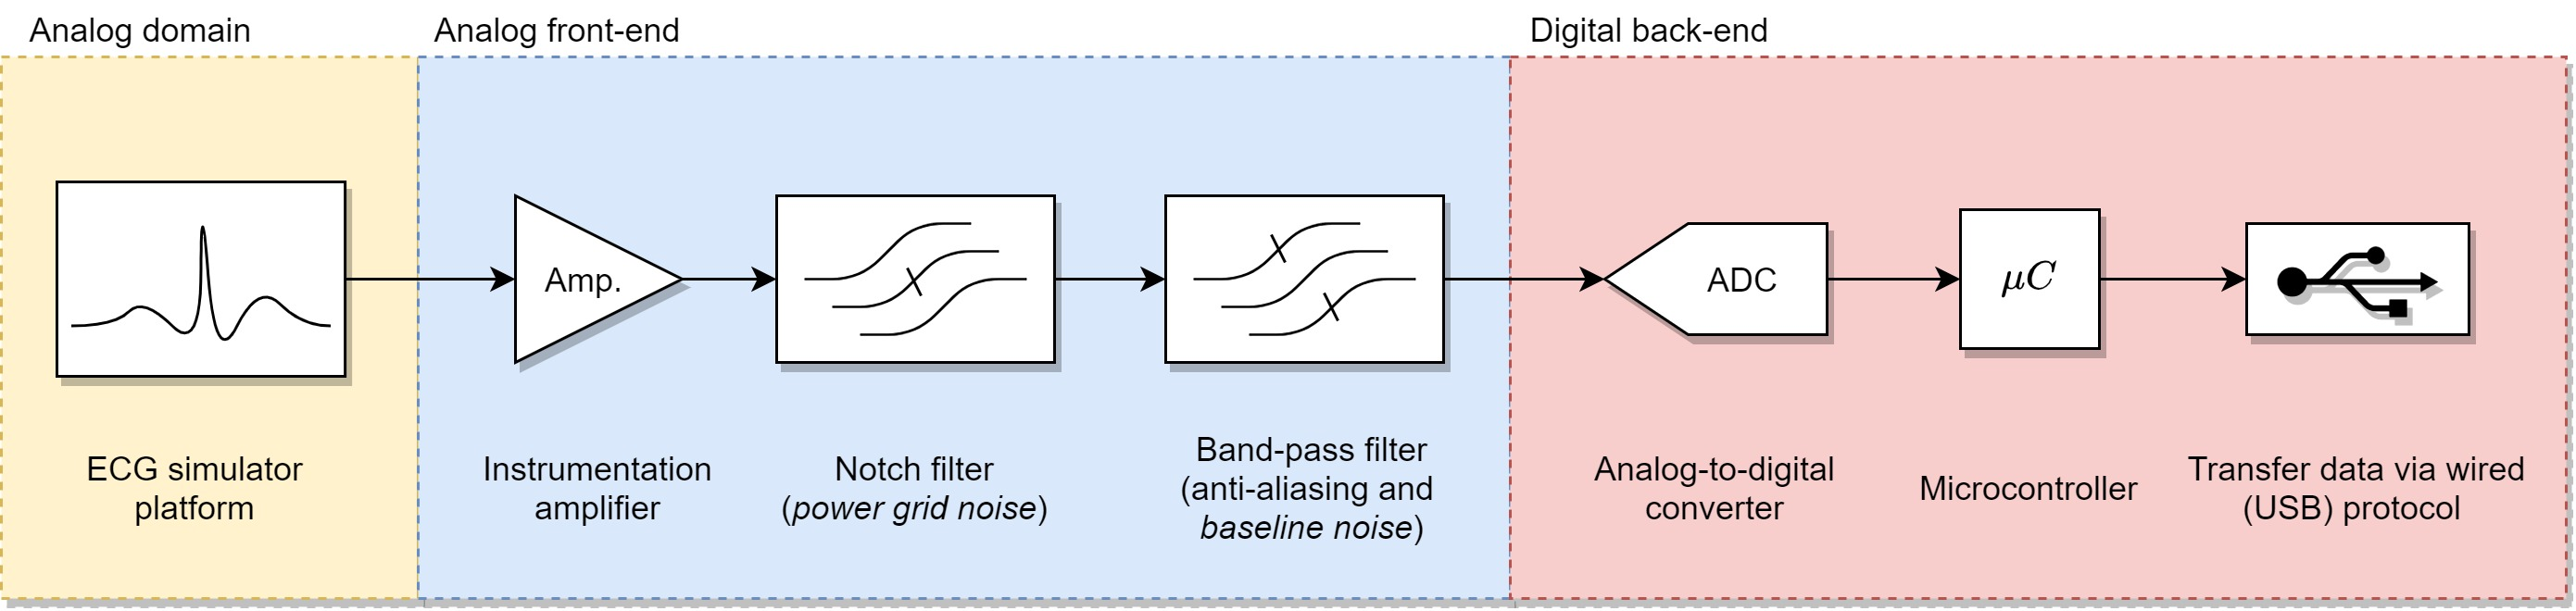
\includegraphics[width=\textwidth,height=\textheight,keepaspectratio]{images/diagram.jpg}
    \caption{Idealized system for acquiring, processing and transferring ECG data.}
    \label{fig:system} 
\end{figure}

The analog front-end contains the preamplifier and filtering. The digital part involves the ADC, signal processing and transmission.

The system analog front-end was entirely tested via the free circuit simulator software LTSpice and all plots were made with the use of the Python Plotly library, since the graphs presented in LTSpice does not have a good quality.

The digital part was simulated with the use of an ECG simulator embedded in an ESP32 outputting via a 8-bit DAC and been collected at a 12-bit ADC in another ESP32. The data was sent to a PC via USB serial connection to by displayed graphically.

\subsection{Preamplifier}

The amplifier architecture used is an instrumentation amplifier of which resembles the topology of a differential amplifiers but with the addition of buffers on each input. The complete circuit can be seen in the figure \ref{ckt:1} below.

\begin{figure}[h!]
\begin{center}
\tikz \node [scale=0.75, inner sep=0] {
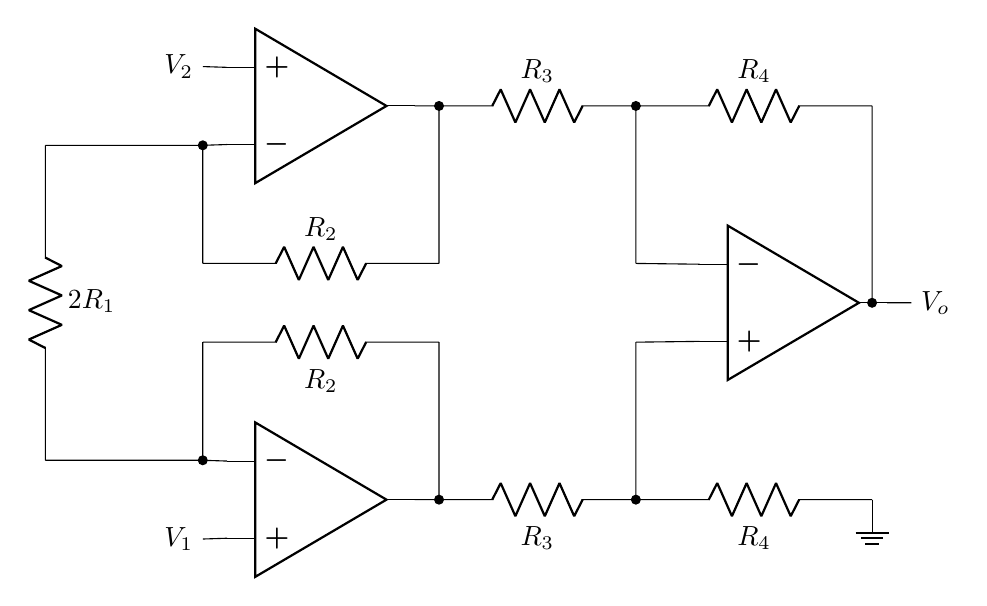
\begin{tikzpicture} [ american, ]
    \draw (-3.5,-3.75) to[R, l_=$2R_1$] (-3.5,0.25) 
    (-3.5,-3.75) to[short,-*] (-1.5,-3.75)
    (-3.5,0.25) to[short,-*] (-1.5,0.25)
    ;
    
    \draw (0,0.75) node[op amp,yscale=-1] (opamp1) {}
    (opamp1.-) -- (-1.5,0.25)
    (opamp1.+) -- (-1.5,1.25)  node[left] {$V_{2}$}
    (opamp1.out) --  (1.5,0.75) %node[right] {$V_o$}
    %(opamp1.up) --++(0,1.005) node[vcc]{15\,\textnormal{V}}
    %(opamp1.down) --++(0,-1.005) node[vee]{-15\,\textnormal{V}}
    (-1.5,0.25) -- (-1.5,-1.25) 
    (-1.5,-1.25) to[R,l=$R_2$] (1.5,-1.25)
    (1.5,-1.25) to[short,-*] (1.5,0.75);
    
    
    \draw (0,-4.25) node[op amp] (opamp2) {}
    (opamp2.+) -- (-1.5,-4.75)  node[left] {$V_{1}$}
    (opamp2.-) -- (-1.5,-3.75)
    (opamp2.out) --  (1.5,-4.25) %node[right] {$V_o$}
    %(opamp2.up) --++(0,0.005) node[vcc]{15\,\textnormal{V}}
    %(opamp2.down) --++(0,-0.005) node[vee]{-15\,\textnormal{V}}
    (-1.5,-3.75) -- (-1.5,-2.25) 
    (-1.5,-2.25) to[R,l_=$R_2$] (1.5,-2.25)
    (1.5,-2.25) to[short,-*] (1.5,-4.25)
    ;
    
    \draw (6,-1.75) node[op amp] (opamp3) {}
    (opamp3.+) -- (4,-2.25)
    (opamp3.-) -- (4,-1.25)
    (opamp3.out) --  (7.5,-1.75) node[right] {$V_o$}
    %(opamp2.up) --++(0,0.005) node[vcc]{15\,\textnormal{V}}
    %(opamp2.down) --++(0,-0.005) node[vee]{-15\,\textnormal{V}}
    ;

    \draw (1.5,0.75) to[R,l=$R_3$, -*] (4,0.75)
    (1.5,-4.25) to[R,l_=$R_3$, -*] (4,-4.25)
    (4,0.75) -- (4,-1.25)
    (4,-4.25) -- (4,-2.25)
    (4,0.75) to[R,l=$R_4$] (7,0.75)
    (4,-4.25) to[R,l_=$R_4$] (7,-4.25)
    (7,-4.25) node[ground]{}
    (7,0.75) to[short,-*] (7,-1.75)
    ;

\end{tikzpicture}
};
\end{center}
\caption{Instrumentation amplifier.}
\label{ckt:1} 
\end{figure}

The output of the instrumentation amplifier can be written as equation \ref{inst:1}:

\begin{center}
\begin{equation} \label{inst:1}
        V_o = \text{DG}(V_1-V_2)+\text{CMG}\left(\frac{V_1+V_2}{2}\right)
\end{equation}
\end{center}

Where $\text{DG}$ is the differential gain and $\text{CMG}$ is the common mode gain given by equations \ref{inst:2} and \ref{inst:3}:

\begin{center}
\begin{equation} \label{inst:2}
    \text{DG} = \frac{R_4}{R_3} \left(1+\frac{R_2}{R_1}\right)
\end{equation}
\end{center}

\begin{center}
\begin{equation} \label{inst:3}
    \text{CMG} = \left(\frac{R_4}{R_3+R_4}\frac{R_1+R_2}{R_1} - \frac{R_2}{R_1}\right)
\end{equation}
\end{center}

In ideal condition the common mode gain is null with the traditional choice of $R_1=R_3$ and $R_2=R_4$, and the final output turns to be $V_o = \text{DG}(V_1-V_2)$.

The problem is that $\text{CMG}$ will never be null due to imprecision in the resistance value of the resistors. Despite this, there is a metric called Common Mode Rejection Ratio (CMRR) given by the equation \ref{inst:4} in dB that indicates how much times higher the differential gain should be relative to the common mode gain. In the case of ECG, this ratio must be higher than $+ 100 \, dB$ \cite{khandpur2019compendium,khandpur2005biomedical}.  Also a input impedance of at least $10 \, M\Omega$ in the input buffers is recommended \cite{khandpur1987handbook}.

\begin{center}
\begin{equation} \label{inst:4}
    \text{CMRR} = 20\text{log}\left(\frac{\text{DG}}{\text{CMG}}\right)
\end{equation}
\end{center}

Usually the differential gain for the preamplifier in a ECG is 500 \cite{khandpur2019compendium}. A better approach would be to distribute this gain along a multistage amplifier to avoid distortion due to non linearities \cite{sedra2020microelectronic}. Despite this statement, the project will be based in a single amplification block for the sake of simplicity, .

The differential gain for the project should be close to 506 with the resistors $R_2=R_4$ with $22 \, k\Omega$ resistors and the resistors $R_1=R_3$ with $1 \, k\Omega$ resistors. 

Considering the gain, the choice of resistors can be illustrated by the table \ref{tbl:2}. Also the operational amplifier LMH6629 \cite{instruments2010lmh6629} was chosen once it is SMD, has ultra-low noise and has a slew rate of $1600 \, V/\mu s$ that can follow the variation of the QRS wave.

\begin{longtable}[H]{lcc}

\toprule
Component & Identifier & Number of components \\
\midrule
\endhead
Resistor & $22 \, k\Omega$ & 4\\
Resistor & $1 \, k\Omega$ & 4\\
Opamp IC & LMH6629 & 3\\
\bottomrule
\caption{Summary of electronic components for the preamplifier.}
\label{tbl:2}
\end{longtable}

\subsection{Analog filters}

\subsubsection{Notch filter}

The Notch filter topology used in this project follows the circuit of figure \ref{ckt:2}. Besides implementing the low-pass and high-pass segment, this filter has a buffer so it isolates from the output and at the end, the output is fed back fractioned to adjust the filter's quality factor (Q).

\begin{figure}[h!]
\begin{center}
\tikz \node [scale=0.75, inner sep=0] {
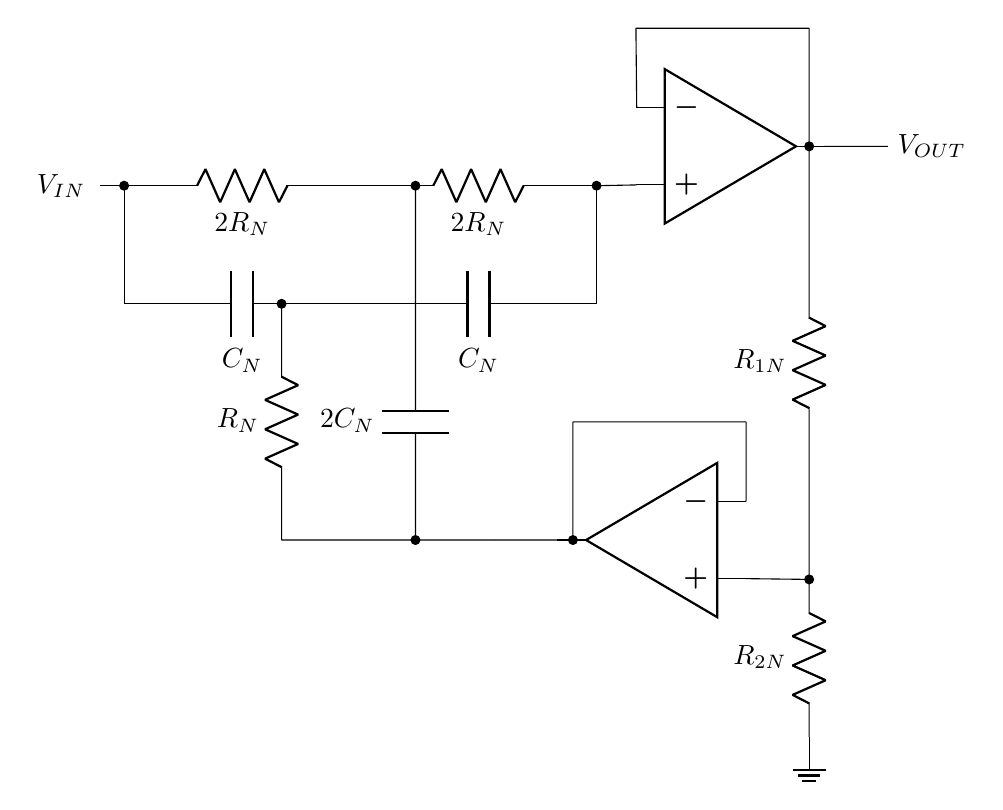
\begin{tikzpicture} [ american, ]
    \draw (0.3,0) -- (0,0) 
    (0.3,0) to[R,l_=$2R_N$, *-] (3.3,0)
    (3.3,0) to[R,l_=$2R_N$, -*] (6.3,0)
    (0.3,0) -- (0.3,-1.5)
    (6.3,0) -- (6.3,-1.5)
    (0.3,-1.5) to[C,l_=$C_N$, -] (3.3,-1.5)
    (3.3,-1.5) to[C,l_=$C_N$, -] (6.3,-1.5)
    (-0.5,0) node[] {$V_{IN}$}
    ;
    
    \draw (2.3,-1.5) to[R,l_=$R_N$, *-] (2.3,-4.5)
    (4,-1.5) to[C,l_=$2C_N$, -*] (4,-4.5)
    (4,0) to[short,*-] (4,-1.5) 
    (2.3,-4.5) -- (5,-4.5)
    ;
    
    
    \draw (8,0.5) node[op amp] (opamp1) {}
    (opamp1.+) -- (6.3,0)  
    (opamp1.-) -- (6.8,2)
    (opamp1.out) --  (10,0.5) node[right] {$V_{OUT}$}
    %(opamp2.up) --++(0,0.005) node[vcc]{15\,\textnormal{V}}
    %(opamp2.down) --++(0,-0.005) node[vee]{-15\,\textnormal{V}}
    (6.8,2) -- (9,2) 
    (9,2) -- (9,0.5)
    (9,0.5) to[R,l_=$R_{1N}$, *-] (9,-5)
    (9,-5) to[R,l_=$R_{2N}$, *-] (9,-7) node[ground] {}
    ;
    
    \draw (7,-4.5) node[op amp, xscale=-1] (opamp2) {}
    (opamp2.+) -- (9,-5) 
    (opamp2.-) -- (8.2,-4)
    (opamp2.out) --  (5,-4.5) 
    (8.2,-4) -- (8.2,-3)
    (8.2,-3) -- (6,-3)
    (6,-3) to[short,-*] (6,-4.5)
    ;


\end{tikzpicture}
};
\end{center}
\caption{Notch filter.}
\label{ckt:2} 
\end{figure}

The cutoff frequency of the previous Notch filter can be found by the equation \ref{notch:1}. Keeping in mind that the cutoff frequency is $60 \, Hz$, the capacitor and resistor could be $100 \, nF$ and $13.2 \, k\Omega$. Once the found resistance does not match with a commercial value, the resistor $R_N$ can be used with a series association of a $13 \, k\Omega$ and $200 \, \Omega$ resistor.

\begin{center}
\begin{equation} \label{notch:1}
    f_c = \frac{1}{4\pi R_N C_N}
\end{equation}
\end{center}

The quality factor (Q) is a function of the cutoff frequency and the bandwidth of the filter, given by the equation \ref{notch:2} where $B_W$ is the bandwidth in Hertz. Setting a bandwidth of 1 Hz with reject band between $59.5$ and $60.5 \, Hz$, which is a band that the power grid voltage can assume in the worst case during anomalies according to \textcite{de2010modulo}. Henceforth the quality factor is found to be $Q=60$ and the remaining resistor can be found by the equation \ref{notch:3} as $R_{1N}=180 \, \Omega$ and $R_{2N}=47 \, k\Omega$.

\begin{center}
\begin{equation} \label{notch:2}
    Q = \frac{f_c}{B_W} 
\end{equation}
\end{center}

\begin{center}
\begin{equation} \label{notch:3}
    1 - \frac{1}{4Q} = \frac{R_{2N}}{R_{2N} + R_{1N}}
\end{equation}
\end{center}

The table \ref{tbl:3} summarizes the components choices for the Notch filter.

\begin{longtable}[H]{lcc}

\toprule
Component & Identifier & Number of components \\
\midrule
\endhead
Resistor & $47 \, k\Omega$ & 1\\
Resistor & $180 \, \Omega$ & 1\\
Resistor & $13 \, k\Omega$ & 5\\
Resistor & $200 \, \Omega$ & 5\\
Capacitor & $100 \, nF$ & 4\\
Opamp IC & LMH6629 & 2\\
\bottomrule
\caption{Summary of electronic components for the Notch filter.}
\label{tbl:3}
\end{longtable}

\subsubsection{Band-pass filter}

Once stated before, the high-pass and low-pass filter were merged into a single band-pass filter. One possible topology for the band-pass filter would be merged a cascade association of a high and low-pass filter, but this choice wastes improvement possibilities. Instead the topology of choice is the one in the figure \ref{ckt:3}

\begin{figure}[h!]
\begin{center}
\tikz \node [scale=0.75, inner sep=0] {
\begin{tikzpicture} [ american, ]
    \draw (0.3,0) to[short,-*] (0,0) 
    (0.3,0) to[R,l_=$R_{B1}$, -] (2.3,0)
    (2.3,0) to[C,l_=$C_{B1}$, -*] (4.3,0)
    (-0.5,0) node[] {$V_{IN}$}
    ;
    
    \draw (6,-0.5) node[op amp] (opamp1) {}
    (opamp1.+) -- (4.3,-1)  
    (opamp1.-) -- (4.3,0)
    (opamp1.out) --  (8.3,-0.5) node[right] {$V_{OUT}$}
    (4.3,-1) -- (4.3,-2) node[ground] {}
    ;
    
    \draw (4.3,1.5) to[R,l_=$R_{B2}$, *-*] (7.2,1.5)
    (4.3,3) to[C,l_=$C_{B2}$, -] (7.2,3)
    (4.3,0) -- (4.3,3)
    (7.2,3) to[short, -*] (7.2,-0.5)
    ;
    


\end{tikzpicture}
};
\end{center}
\caption{Band-pass filter.}
\label{ckt:3} 
\end{figure}

The filter stated above is an inverting active band-pass filter. Its equations are: equation \ref{band:2} to select the gain between input and output, which in this case will be set to one, resulting in $R_{B1} = R_{B2}$; equation \ref{band:3} to select the capacitance of $C_{B1}$ based in the lower cutoff frequency ($f_L = 0.5 \, Hz$); and equation \ref{band:4} regarding $C_{B2}$ based in the higher cutoff frequency ($f_H = 200 \, Hz$).

\begin{center}
\begin{equation} \label{band:2}
    \text{Gain} = A_v = - \frac{R_{B2}}{R_{1B}}
\end{equation}
\end{center}

\begin{center}
\begin{equation} \label{band:3}
    f_L = \frac{1}{2\pi R_{B1}C_{B1}}
\end{equation}
\end{center}

\begin{center}
\begin{equation} \label{band:4}
    f_H = \frac{1}{2\pi R_{B2}C_{B2}}
\end{equation}
\end{center}

An inverting amplifier with unitary gain can be placed in the output of the band-pass filter to correct the polarity of the resulting signal, or instead just inverting when taking the output between $V_{OUT}$ and ground node.

The values found for the components are summarized in the table \ref{tbl:4}, considering $R_{B1}=R_{B2}=500 \, k\Omega$, $C_{B1}=636 \, n F$ and $C_{B2} = 1.59 \, n F$. The capacitor $C_{B1}$ was broken into a parallel association of four capacitors $0.22 \mu F$, $0.22 \mu F$, $0.18 \mu F$, $0.015 \mu F$ and $0.001 \mu F$. The same for $C_{B2}$ but with a parallel association of $680 p F$, $680 p F$, $220 p F$ and $10 p F$.

\begin{longtable}[H]{lcc}

\toprule
Component & Identifier & Number of components \\
\midrule
\endhead
Resistor & $500 \, k\Omega$ & 2\\
Capacitor & $0.22 \, \mu F$ & 2 \\
Capacitor & $0.18 \, \mu F$ & 1 \\
Capacitor & $0.015 \, \mu F$ & 1 \\
Capacitor & $0.001 \, \mu F$ & 1 \\
Capacitor & $680 \, pF$ & 2\\
Capacitor & $220 \, pF$ & 1\\
Capacitor & $10 \, pF$ & 1\\
Opamp IC & LMH6629 & 1\\
\bottomrule
\caption{Summary of electronic components for the band-pass filter.}
\label{tbl:4}
\end{longtable}

\subsection{ECG simulator}

Prior to the tests of the digital processing algorithms, there is a need to simulate typical ECG signal with a good model in the software domain. The high level abstraction allow it to debug faster than deploying and testing direct in the hardware.

The model used was the one presented by \textcite{quiroz2019generation}, whose consists in the use of three different nonlinear oscillators related to the cardiac natural pacemakers where three coupled oscillators represent the action potentials of the SA node, AV node and His-Purkinje complex, as illustrated in the figure \ref{fig:simulate} extracted from \textcite{quiroz2019generation}.

\begin{figure}[h!] 
    \centering
    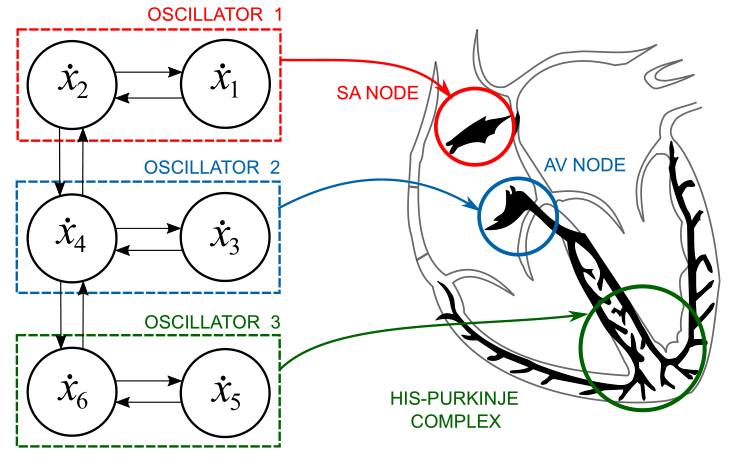
\includegraphics[width=9cm]{images/oscillators.png}
    \caption{Diagram relating the cardiac natural pacemakers to non linear variables. Source: \textcite{quiroz2019generation}.}
    \label{fig:simulate}
\end{figure}

\textcite{quiroz2019generation} also derive an ODE system of nonlinear equations to represent the given oscillators, as illustrated in the equation \ref{sim:1}.

\begin{center}

\begin{equation} \label{sim:1}
\centering
\begin{cases}
    \dot{x_1} = \Gamma_t \cdot (x_1 - x_2 - Cx_1x_2 - x_1x_2^2) \\
    \dot{x_2} = \Gamma_t \cdot (Hx_1 - 3x_2 + Cx_1x_2 + x_1x_2^2 + 2 \beta(x_4-x_2)) \\
    \dot{x_3} = \Gamma_t \cdot (x_3 - x_4 - Cx_3x_4 - x_3x_4^2) \\
    \dot{x_4} = \Gamma_t \cdot (Hx_3 - 3x_4 + Cx_3x_4 + x_3x_4^2 + 2 \beta(x_2-x_4)) \\
    \text{ECG}(t) = \alpha_1 x_1 + \alpha_2 x_2 + \alpha_3 x_3 + \alpha_4 x_4
\end{cases} 
\end{equation}
\end{center}

The whole description is left for the original paper, but is known that a correct choice of the coefficients results in changes in the ECG waveform. \textcite{quiroz2019generation} comes with a set of coefficients that calibrates the ECG in different modes, varying from the normal cardiac rhythm and also represent pathologies such as: sinus tachycardia, atrial flutter, ventricular tachycardia and ventricular flutter. The table \ref{tbl:5} illustrates the coefficients used by \textcite{quiroz2019generation} to generate each mode, starting from the initial excitation of $\textbf{x} = \{0, 0, 0.1, 0\}$.

\begin{longtable}[H]{lcccccc}

\toprule
Mode & $H$ & $\Gamma_t$ & $\alpha_1$ & $\alpha_2$ & $\alpha_3$ & $\alpha_4$\\
\midrule
\endhead
Normal rhythm & 3 & 7 & -0.024 & 0.0216 & -0.0012 & 0.12 \\
Sinus tachycardia & 2.848 & 21 & 0 & -0.1 & 0 & 0 \\
Atrial flutter & 1.52 & 13 & -0.068 & 0.028 & -0.024 & 0.12 \\
Ventricular tachycardia & 2.178 & 21 & 0 & 0 & 0 & -0.1 \\
Ventricular flutter & 2.178 & 13 & 0.1 & -0.02 & -0.01 & 0 \\
\bottomrule
\caption{Coefficients for the ECG simulator to access each mode. The coefficients $C=1.35$ and $\beta=4$ are constants along all the simulations. Source: adapted from \textcite{quiroz2019generation}.}
\label{tbl:5}
\end{longtable}

With this representation, a code in Python was created to simulate the ECG in software and further a firmware for the Espressif micro controller ESP32 was also created, allowing the internal 8-bit DAC (digital-to-analog converter) to continuously output the ECG simulation given by the model above. It was also predict a switch button in the micro controller to switch between each pathology. In both cases a fixed sampling period of $10^{-4}$ was used. The simulation results will be shown in further sections.

The analog front-end simulations has an ECG simulator implemented via piece-wise linear voltage source with a predefined ECG waveform.

\subsection{ECG signal processing}

The main objective of the micro controller is to implement signal processing algorithms to extract information from the ECG signal. But before the actual hardware implementation, those routines were tested in a high level of abstraction in Python.

Before any processing in the micro controller it was implemented an moving average filter of arbitrary size of 16 samples to filter the noise in the incoming signal. 

\subsubsection{Heart rate detection}

The algorithm design to detect the hear rate is a simply detection of the peak in the QRS complex followed by the time distance between QRS peaks. The steps in the calculation is as follows:

\begin{itemize}
    \item Window a portion of the signal (buffer);
    \item Set a proper threshold in amplitude to detect the peaks in the QRS complex, it was used a threshold of 90\% of the ECG maximum amplitude, but a value of 130\%-140\% of the RMS value of the buffer might be used;
    \item Proceed to peak detection where:
    \begin{itemize}
        \item The ECG signal is evaluated if its amplitude overtakes the threshold value;
        \item Considering values that meet the overrun criterion, those are tracked to monitor any amplitude rising;
        \item If the amplitude is rising, it is tracked the inflection point where the signal transits from rising to decreasing;
        \item Thus the inflection point is the peak of the QRS complex;
    \end{itemize}
    \item During the peaks detection the time interval between peaks are calculated, thus its inverse giving the heart rate.
\end{itemize}

The heart rate detection algorithm was first implemented in high level of abstraction in Python using the ECG generator previously stated, so after the tests it can be safely implemented in a hardware manner. The tests results are displayed in the results section.

\subsubsection{Pathology analysis}

The pathology analysis is based in the results obtained for the heart rate (that involves time intervals, duration and location) out of the expected values of 60 to 100 bpm (considering that the ECG is measured with a patient at rest) and also amplitude extremes and variations \cite{kherabnormality, stuchilin2017use, clevelandclinic}.

During the test for pathologies it is important to make use of the ECG generator outputting wave forms that are not in the normal rhythm, i.e. sinus tachycardia, atrial flutter, ventricular tachycardia and ventricular flutter.

\subsection{ECG embedded acquisition system}

The main block of the system is the ESP32 responsible to collect data at a sampling rate of $500 \, Hz$, process the signal to extract further information and transmits the data to the ECG viewer.

The data was collected with the ESP32 built-in 12-bit SAR ADC. The linear range of this ADC is adjustable according to the attenuation. Considering an attenuation of 11dB, the possible range of voltages in the ADC input varies from 150 to 2450 mV. The DAC output was configured so the voltage does not fall of this range, causing distortion due to non-linearities in the ADC.

The firmware code structure is based in the freeRTOS, using tasks and event groups to handle the tasks access. In total there are five tasks in the code, each one responsible for:

\begin{itemize}
    \item Start the data acquisition;
    \item Finish the data acquistion and returning to idle mode, waiting for another session to start;
    \item Record data from ADC into a buffer;
    \item Apply the digital signal processing algorithms previous discussed in the data inside the ADC buffer and store in another buffer (DSP buffer);
    \item Finally, transmit via USB serial the content inside the DSP buffer;
\end{itemize}

Once the ESP32 has two cores, the ADC task was assigned to the core number 1 and all other were assigned to the core 0. This allows for the data to be acquired continuously without interference of another task.

Despite the efforts to feed the DAQ via the ESP32 ECG simulator, due to lack of resources, the signal is not well conditioned, so the solution for the simulations is to merge the both the simulator and the DAQ in a single micro controller to test the signal processing algorithms. Noise was inserted in the generation to simulate the conditions in a real acquisition.

\subsection{ECG viewer}

The ECG viewer platform was design as a Python application running in a PC that receives serial data from the ESP32 DAQ and plots the ECG amplitude in real-time.

Acquired data is also stored in a \texttt{.csv} file.

\pagebreak
\section{Results}

\lipsum[1]

\pagebreak
\section{Discussions}

\lipsum[1]

\pagebreak
\section{Conclusions}

\lipsum[1]

\pagebreak
    \appendix
\section{Schematics}
\pagebreak



\end{document}